\subsubsection{UC5.1 - Inserimento credenziali di accesso }
\begin{figure}[h]
	\centering
	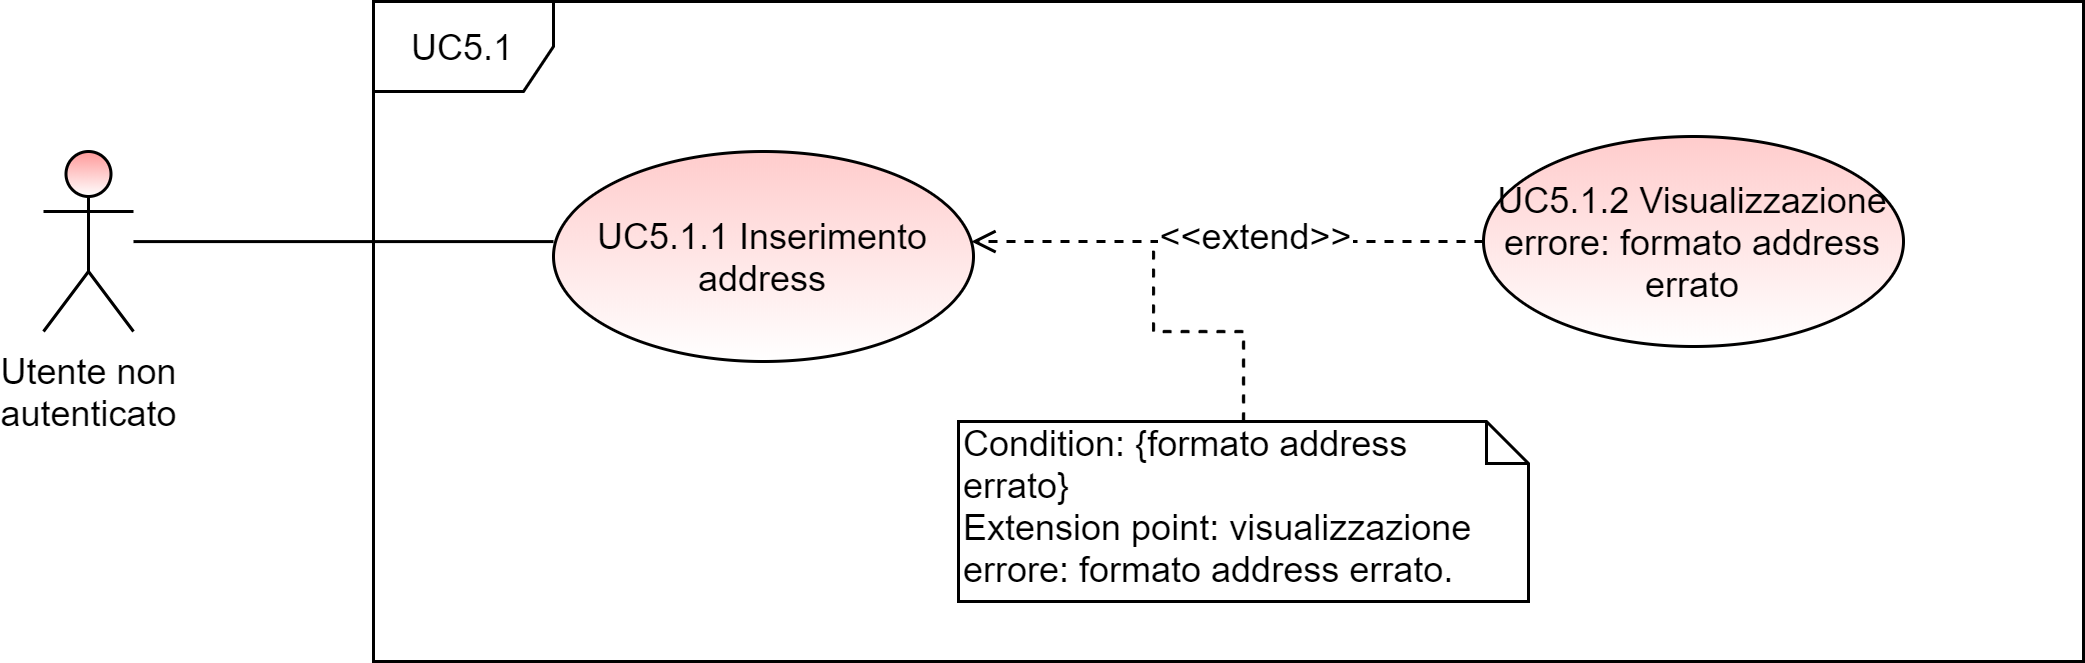
\includegraphics[scale=\ucs]{./res/img/UC5.1.png}
	\caption {UC5.1 - Inserimento credenziali di accesso }
\end{figure}
\begin{itemize}
	\item \textbf{Attori primari:} \una{};
	\item \textbf{Attori secondari:} \re{};
	\item \textbf{Descrizione:} l’utente procede all’inserimento delle credenziali necessarie per l'autenticazione. Oltre all’inserimento obbligatorio dell’address viene richiesta, a scelta dell’utente, la private key\ped{\textit{G}} o mnemonic phrase\ped{\textit{G}}; 
	\item \textbf{Scenario principale:} l'utente provvede ad inserire le credenziali necessarie per l’accesso.  
	\item \textbf{Specializzazioni:} 
	\begin{itemize}
		\item \textbf{UC5.2:} l’utente decide di eseguire il login tramite private key\ped{\textit{G}};
		\item \textbf{UC5.3:} ’utente decide di eseguire il login tramite mnemonic phrase\ped{\textit{G}}.
	\end{itemize}
	\item \textbf{Estensioni:} 
	\begin{itemize}
		\item \textbf{UC5.6:} se le credenziali inserite sono errate allora il sistema mostra un messaggio di errore.  
	\end{itemize}
	\item \textbf{Precondizione:}  l’utente ha inserito il comando \login{};   
	\item \textbf{Postcondizione:} l'utente ha inserito correttamente le credenziali per effettuare l’accesso. 
\end{itemize}